%\documentclass[english, times, mirror]{revdetua}
% use this if you're writing in portuguese:
\documentclass[portuguese, times, mirror]{revdetua}

\usepackage[utf8]{inputenc}
\usepackage{graphicx}
\usepackage{hyperref}

\usepackage{amsmath}
\usepackage{mathtools}

\usepackage{caption}
\usepackage{listings}
\usepackage{color}

\definecolor{dkgreen}{rgb}{0,0.6,0}
\definecolor{gray}{rgb}{0.5,0.5,0.5}
\definecolor{mauve}{rgb}{0.58,0,0.82}

\lstset{frame=tb,
  language=Java,    
  aboveskip=3mm,
  belowskip=3mm,
  showstringspaces=false,
  columns=flexible,
  basicstyle={\small\ttfamily},
  numbers=none,
  numberstyle=\tiny\color{gray},
  keywordstyle=\color{blue},
  commentstyle=\color{dkgreen},
  stringstyle=\color{mauve},
  breaklines=true,
  breakatwhitespace=true,
  tabsize=3
}

\usepackage{tikz}
\usepackage{pgfplots}

% correct bad hyphenation here
\hyphenation{op-tical net-works semi-conduc-tor}

\begin{document}

\Header{1}{5}{Outubro}{2016}{1}
% Note: the month must be in Portuguese

\title{Visão por Computador 2016-17, Guia Prático N.º 6}
\author{Rui Oliveira, Tomás Rodrigues\\ DETI, Universidade de Aveiro \\ Aveiro, Portugal \\ \{ruipedrooliveira, tomasrodrigues\}@ua.pt}
% you should be able to use the \and keyword, but the deti format doesn't like it, for some reason
\maketitle

\begin{resumo}


Pretende-se através deste relatório expor sob forma escrita, o nosso desempenho e objetivos alcançados na aula prática n.º 6 da unidade curricular de Visão por Computador do Mestrado Integrado de Engenharia de Computadores e Telemática.

Neste relatório pretenderemos explicar as soluções por nós encontradas para a resolução dos diferentes problemas propostos.


\end{resumo} 

\begin{palavraschave} %
visão, computador, imagem digital, stereo calibration, opencv, c++, 
 \end{palavraschave} %




\section{Repositório: código fonte}


Todas as soluções dos problemas propostos estão disponível através do seguinte repositório (gitHub) criado para o efeito. \\

\href{http://github.com/toomyy94/CV1617-68779-68129}{http://github.com/toomyy94/CV1617-68779-68129}
\\


A resolução dos problemas do presente guia encontram-se na pasta aula6. Para a resolução dos exercícios foi usado o \texttt{Code::Blocks IDE}. 



\section{Problemas propostos}



\subsection{Problema \#1 - \textit{Chessboard calibration}}

\subsubsection{Enunciado}
\textit{Compile and test the file chessboard.cpp (similar to the one used in the last lecture). Fill the necessary matrices with the correct value to calibrate the stereo pair. Analyze the code for filling the 3D coordinates of the pattern.}


\subsubsection{Resolução e principais conclusões}

Efetuando umas ligeiras alterações ao código para o nosso IDE conseguimos compilá-lo e detetamos os cantos com a função \texttt{FindAndDisplayChessboard} da seguinte forma: 

\begin{lstlisting}[caption=Função contagem dos cantos,label=code:C]
// find and display corners
corner_count = FindAndDisplayChessboard(image,board_w,
        board_h,&corners);
\end{lstlisting}


\begin{figure}[ht!]
\centering
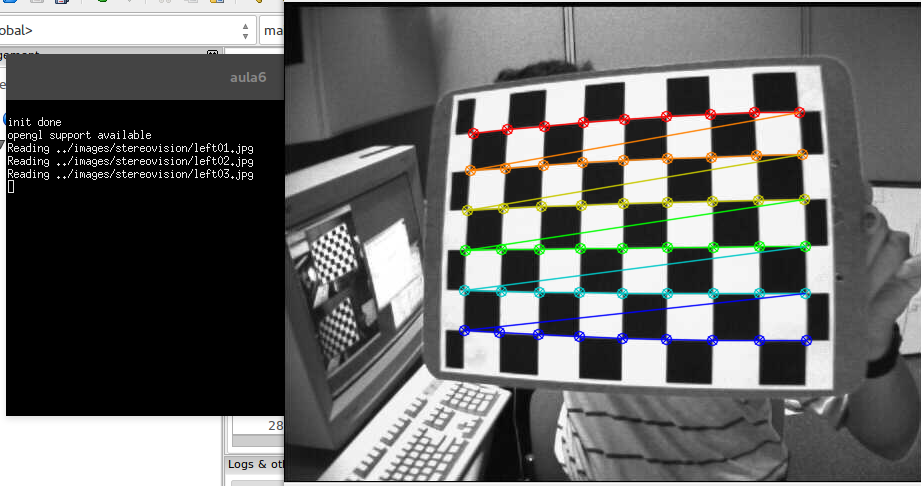
\includegraphics[width=70mm]{img/ex1.png}
\caption{Resultado obtido após exercício 1}
\end{figure}



\subsection{Problema \#2 - \textit{Stereo calibration}}

\subsubsection{Enunciado}
\textit{Calibrate the stereo pair using the function cvStereoCalibrate. After a successful calibration, save the matrices in an xml file using the file storage functions to
avoid recalibration of the stereo rig each time.}

\subsubsection{Resolução e principais conclusões}

Primeiramente calibramos a câmara para cada par de duas imagens dadas desta maneira:

\begin{lstlisting}[caption=Função streoCalibrate,label=code:C]

Mat R, T, E, F;

double rms = stereoCalibrate(object_points, image_pointsL, image_pointsR,
cameraMatrix1, distCoeffs1,
cameraMatrix2, distCoeffs2,
imageL.size(), R, T, E, F,
TermCriteria(CV_TERMCRIT_ITER+CV_TERMCRIT_EPS, 50, 1e-6),
CV_CALIB_FIX_FOCAL_LENGTH );
\end{lstlisting}

De seguida gravámos os parâmetros indicados no XML com o código fornecidoe escrevemos a matriz associada com os seus valores intrisecos, como se pode ver na imagem seguinte: 

\newpage

\begin{figure}[ht!]
\centering
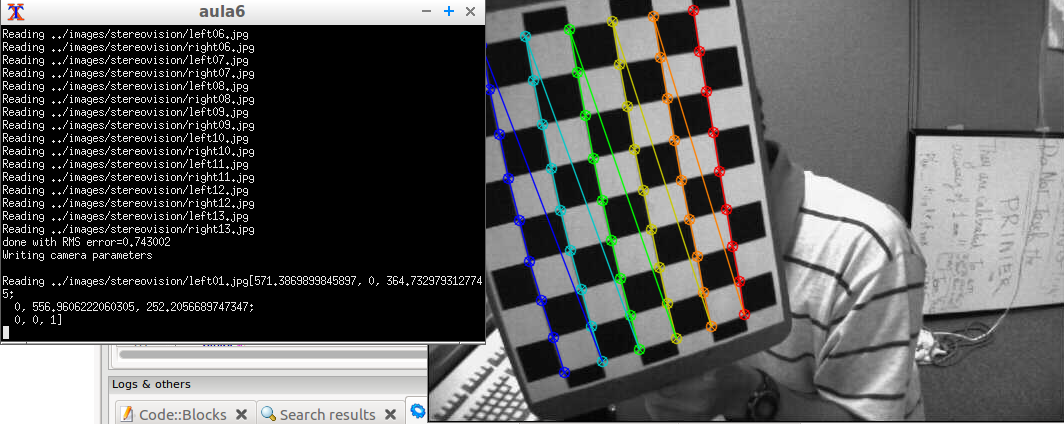
\includegraphics[width=70mm]{img/ex2.png}
\caption{Resultado obtido após exercício 2}
\end{figure}

De seguida, encontra-se um excerto do ficheiro XML gerado. 


\begin{lstlisting}[caption=Ficheiro XML gerado,label=code:C]

<?xml version="1.0"?>
<opencv_storage>
<cameraMatrix_1 type_id="opencv-matrix">
  <rows>3</rows>
  <cols>3</cols>
  <dt>d</dt>
  <data>
    5.7138698998458972e+02 0. 3.6473297931277449e+02 0.
    5.5696062220603051e+02 2.5220566897473466e+02 0. 0. 1.</data></cameraMatrix_1>
<distCoeffs_1 type_id="opencv-matrix">
  <rows>1</rows>
  <cols>5</cols>
  <dt>d</dt>
  <data>
    -2.5451629689067001e-01 1.9279241569751074e-01
    -1.6798462796271199e-03 2.3027436119502927e-02
    -1.2838981716204551e-01</data></distCoeffs_1>
<cameraMatrix_2 type_id="opencv-matrix">
  <rows>3</rows>
  <cols>3</cols>
  <dt>d</dt>
  <data>
    5.5994944648413571e+02 0. 3.5082756593670024e+02 0.
    5.6302127613737832e+02 2.3385777469609181e+02 0. 0. 1.</data></cameraMatrix_2>
<distCoeffs_2 type_id="opencv-matrix">
  <rows>1</rows>
  <cols>5</cols>
  <dt>d</dt>
  <data>
    -4.8570573185961191e-01 1.7475908406455720e+00
    4.9687215534607008e-04 1.3814048691405257e-03
    -3.9846820537322838e+00</data></distCoeffs_2>
    
\end{lstlisting}


%%%%%%%%%%%%%%%%%%%%%%%%%%%%%%%%%


\subsection{Problema \#3 - \textit{Lens distortion}}

\subsubsection{Enunciado}
\textit{In a new file, read the distortion parameters of the cameras (function cvLoad ), select a stereo pair of
images from the pool of calibration images and present the undistorted images (image with the lens
distortion removed) using the function cvUndistort to compute the new images.}

\subsubsection{Resolução e principais conclusões}

Neste exercício é pedido para retirar a distorção produzida pelas lentes da câmara. Após gravar os parâmetros no XML como referido acima no exercício 2 usamos a função \texttt{cvUndistort} com o código abaixo mostrado, produzindo o seguinte resultado.

\begin{lstlisting}[caption=Função undistrort,label=code:C]
Mat imageUndistortedL;
for (i=0;i<1;i++){
    // read image
    sprintf(filename,"../images/stereovision/
        left\%02d.jpg",i+1);
    printf("\nReading \%s",filename);
    imageL = cv::imread(filename, CV_LOAD_IMAGE_COLOR);

    undistort(imageL, imageUndistortedL, cameraMatrix1, distCoeffs1);

}
std::cout << cameraMatrix1 << std::endl;

imshow("output", imageL);
imshow("undistorted", imageUndistortedL);
\end{lstlisting}

Como conclusão consegue-se observar na imagem sem distorção das lentes que em especial as bordas do \texttt{chessboard} parecem muito mais retas, semelhantes à realidade. Vemos que na imagem do lado estas mesmas bordas têm uma saliência curva o que já quase não se verifica na imagem sem distorção (imagem à direita).


\begin{figure}[ht!]
\centering
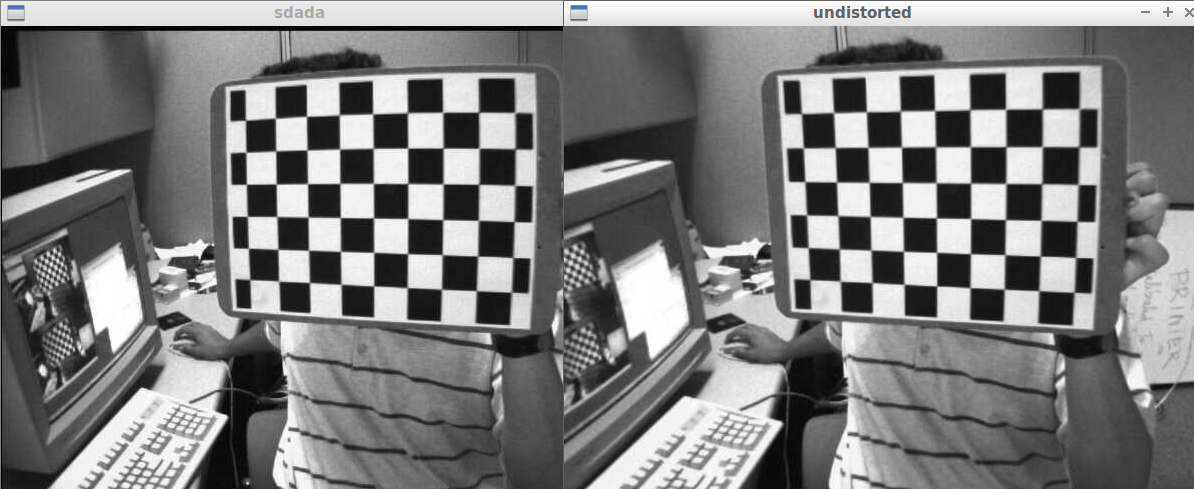
\includegraphics[width=70mm]{img/ex3.png}
\caption{Resultado obtido após exercício 3}
\end{figure}


%%%%%%%%%%%%%%%%%%%%%%%%%%%%%%%%%


\subsection{Problema \#4 - \textit{Epipolar lines}}

\subsubsection{Enunciado}
\textit{Modify the previous example to show only the undistorted images. Add the possibility to select a
pixel in each image using the following code to set a callback to be called for handling mouse events.}

\subsubsection{Resolução e principais conclusões}

Temos um \textit{callback} para determinar as coordenadas dos píxeis da imagem. 

\begin{figure}[ht!]
\centering
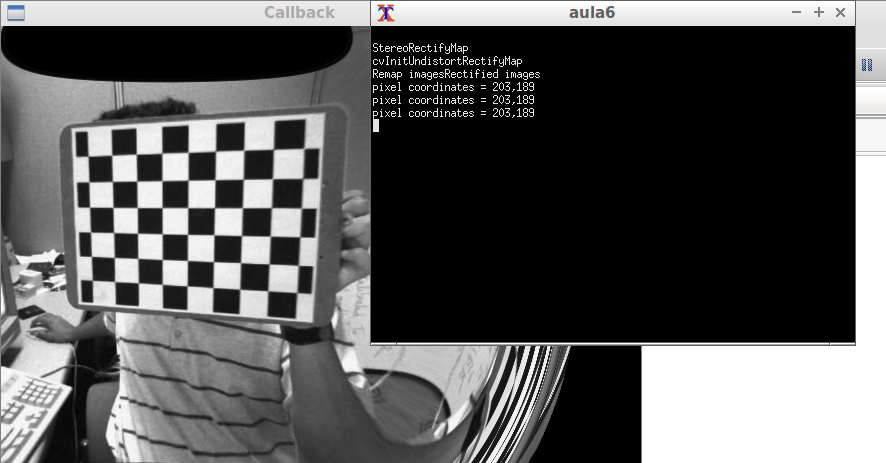
\includegraphics[width=70mm]{img/ex4.png}
\caption{Resultado obtido após exercício 4}
\end{figure}

%%%%%%%%%%%%%%%%%%%%%%%%%%%%%%%%%

\subsection{Problema \#5 - \textit{Image rectification}}

\subsubsection{Enunciado}
\textit{Select a pair of stereo images and use the following OpenCV functions to generate the rectified images (corresponding epipolar lines in the same rows in both images). Visualize the resulting images, and draw lines in rows (for example at each 25 pixels) to evaluate
visually if corresponding pixels are in corresponding lines.}

\subsubsection{Resolução e principais conclusões}

Usámos dois \textit{callbacks} neste exercício para determinar as coordenadas dos píxeis da imagem da esquerda e direita. Distinguindo-os como se pode ver na imagem abaixo.

\begin{figure}[ht!]
\centering
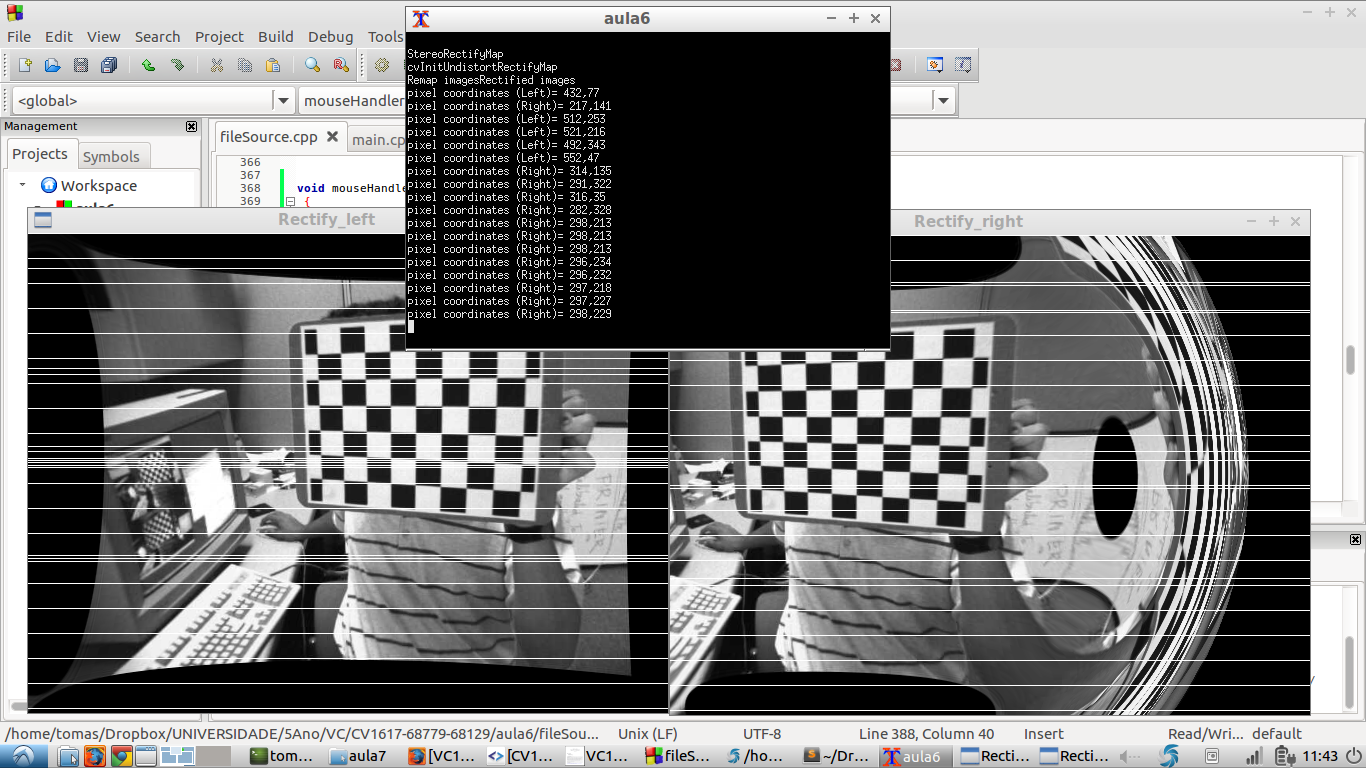
\includegraphics[width=70mm]{img/ex5.png}
\caption{Resultado obtido após exercício 5}
\end{figure}


As linhas são desenhadas com recurso à função \texttt{cv:line} na imagem \texttt{rectified} correspondente.

\begin{lstlisting}[caption=Função mouseHAndler,label=code:C]
void mouseHandlerL(int event, int x, int y, int flags, void* param){
    switch(event){
        case CV_EVENT_LBUTTONDOWN:
        cv::Mat* image = (cv::Mat*) param;
        std::cout << "pixel coordinates (Left)= " << x << "," << y << std::endl;
        std::vector<cv::Point2f> point;
        cv::line(*image,cvPoint(0,y),cvPoint(image
            ->size().width,y),cvScalar(255), 1, 8, 0);
        cv::imshow("Rectify_right",*image);
        break;
    }
}
\end{lstlisting}

Todo o processamento anterior é feito desta maneira, tanto para a imagem da esquerda como para a da direita. 

\begin{lstlisting}[caption=Função Rectify e remap,label=code:C]
std::cout << "\nStereoRectifyMap";
cv::stereoRectify(intrinsics1, distortion1, intrinsics2, distortion2, imagel.size(), rotation, translation,R1, R2, P1, P2, Q,0);

std::cout << "\ncvInitUndistortRectifyMap";
cv::initUndistortRectifyMap(intrinsics1, distortion1, R1, P1, imagel.size(), CV_32FC1, map1x, map1y);
cv::initUndistortRectifyMap(intrinsics2, distortion2, R2, P2, imagel.size(), CV_32FC1, map2x,map2y);

std::cout << "\nRemap images";
cv::Mat  gray_imagel;
cv::Mat  remap_imgl;
cv::cvtColor(imagel, gray_imagel , CV_RGB2GRAY);
cv::remap(gray_imagel, remap_imgl, map1x, map1y,cv::INTER_LINEAR, cv::BORDER_CONSTANT, cv::Scalar());
\end{lstlisting}


\begin{thebibliography}{1} % 9



\bibitem{fsound}
Neves, A. J. R.; Dias, P. Slides teóricos Visão por Computador - Aula 6 (2016)


\bibitem{vtk}
OpenCV. \href{hhttp://docs.opencv.org/}{Opencv Documentation}. Web. 5 Novembro 2016. 




\end{thebibliography}

\end{document}
